\begin{activity} \label{A:10.6.10} 
  Let's consider the function $f$ defined  by $f(x,y) = x^2 - y^2$.  Some contours for this function are shown in Figure
  \ref{F:10.6.activity.1}. 

  \begin{figure}[ht]
    \begin{center}
      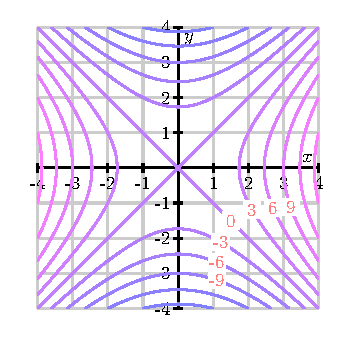
\includegraphics{figures/fig_10_6_contours_1.eps}
    \end{center}	
    \caption{Contours of $f(x,y) = x^2 - y^2$. }
    \label{F:10.6.activity.1}
  \end{figure}
  \ba
  \item Find the gradient $\nabla f (x,y)$.
  \item For each of the following points $(x_0,y_0)$, evaluate the gradient $\nabla f(x_0,y_0)$ and sketch the gradient vector with its tail at
    $(x_0,y_0)$.  Some of the vectors are too long
    to fit onto the plot, but we'd like to draw them to scale;  to do so, scale each vector by a factor of 1/4.
    \begin{itemize}
      \item $(x_0,y_0) = (2,0)$
      \item $(x_0,y_0) = (0,2)$
      \item $(x_0,y_0) = (2,2)$
      \item $(x_0,y_0) = (2,1)$
      \item $(x_0,y_0) = (-3,2)$
      \item $(x_0,y_0) = (-2,-4)$
      \item $(x_0,y_0) = (0,0)$
    \end{itemize}
  \item What do you notice about the relationship between the gradient at
    $(x_0,y_0)$ and the contour line passing through that point?
  \item Does $f$ increase or decrease in the direction of $\nabla
    f(x_0,y_0)$?  Provide a justification for your response.

    \ea

\end{activity}

\begin{activitySolution}
\ba 
\item By definition, 
\[\nabla f (x,y) = \langle f_x(x,y), f_y(x,y) \rangle = \langle 2x, -2y \rangle.\]

\item We apply the formula for the gradient to see that 
\begin{align*}
\nabla f(2,0) &= \langle 4,0 \rangle \\
\nabla f(0,2) &= \langle 0,-4 \rangle \\
\nabla f(2,2) &= \langle 4,-4 \rangle \\
\nabla f(2,1) &= \langle 4,-2 \rangle \\
\nabla f(-3,2) &= \langle -3,-4 \rangle \\
\nabla f(-2,-4) &= \langle -4,8 \rangle \\
\nabla f (0,0) &= \langle 0,0 \rangle.
\end{align*}
A picture of the scaled gradients are shown here. 
   \begin{center}
      \resizebox{!}{2.4in}{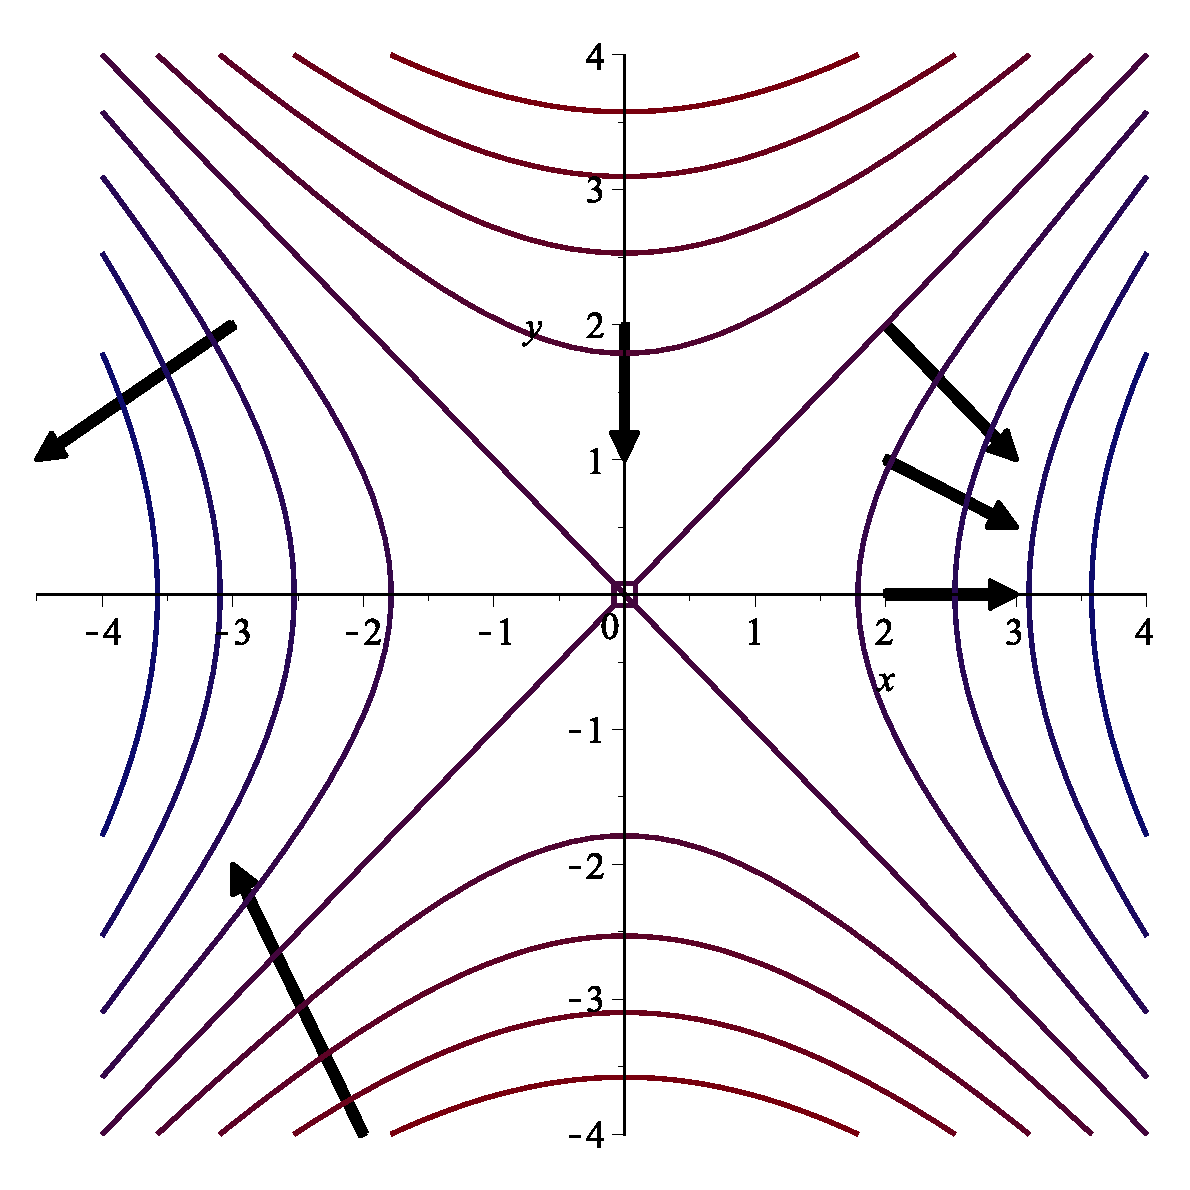
\includegraphics{figures/fig_10_6_Act_10_contours.eps}}
    \end{center}
\item It appears that each gradient is orthogonal to the contour containing its tail.
\item In the first quadrant, as $x$ increases so does $f(x,y)$. So these gradients all point in a direction of increase of $f$. In the second quadrant, as $x$ decreases $f(x,y)$ increases. So these gradients all point in a direction of increase of $f$. In the third quadrant, as $y$ increases so does $f(x,y)$. So these gradients all point in a direction of increase of $f$. Finally, at the point $(0,2)$, $f$ increases as $y$ decreases. So every gradient points in a direction of increase of $f$.
\ea
 
\end{activitySolution}
\aftera
